\documentclass[../DraftNotes.tex]{subfiles}

\begin{document}

The in class work mainly focused on the deployment of functions. As said, the main functionality provided by FogFaas is the secure deployment of functions on an infrastructure: to get this, we provide a \emph{placeApp} predicate. As an app is a list of services, the predicate call internally the \emph{placeService} predicate, which in turn calls the \emph{placeFunctions} one. Here (parallel or sequential) functions are deployed, according to the resources and the security guarantees of the nodes.
The codebase also embed the trust model of SecFog and can be customized with different trust models. Except for this, basic functionalities of FogFaas don't require a probabilistic reasoning (while, as we'll see in the following, probability plays a key role in modelling communication). \\
In this preliminary work, we had a quite simple type system and few language constructs. The language has been later extended with several instructions, as well as for the type system which provides some new rules.

\subsection{Example: testing FogFaas basic functionalities}
As a main example, we provide a set of services and a complete lattice (in particular a strict total order) as a labelling, as shown in fig.~\ref{fig:tot_order}.

\begin{figure}[h!]
	\begin{center}
	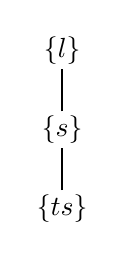
\begin{tikzpicture}
    	\node (top) at (0,0) {$\{ts\}$};
    	\node (med) at (0,1) {$\{s\}$};
    	\node (bot) at (0,2) {$\{l\}$};
    	\draw [thick, shorten <=-2pt, shorten >=-2pt] (top) -- (med);
    	\draw [thick, shorten <=-2pt, shorten >=-2pt] (med) -- (bot); 
	\end{tikzpicture}
	\caption{Default lattice}
  	\label{fig:tot_order}
  	\end{center}
\end{figure}

This can be easily defined by the user by providing a suitable definition of the \emph{labelF} predicate as follows:

\begin{verbatim}
	labelF(ann, Args, ts).
	labelF(ann, Args, s) :- 
                    findall(X, ts(X, Args), []).
	labelF(ann, Args, l) :- 
                    findall(X, notPublic(X, Args), []).
\end{verbatim}

As we'll see, more complicated structures can be provided in a similar way: more on this later on. \\
In this case, we just state that
\begin{itemize}
	\item any function can be top secret (in some sense, low level information can always be promoted to a higher level),
	\item a function can be secret iff it does not have top secret arguments,
	\item a function can be low iff it does not have top secret or secret arguments.
\end{itemize}

\end{document}